1% 
% Lecture Template for ME3023 -  Measurements in Mechanical Systems - Tennessee Technological University
%
% Spring 2020 - Summer 2020
% Tristan Hill, May 07, 2020 - June 12, 2020
% Module 4 - Strain Gauges
% Topic 2 - The Wheatstone Bridge
%

\documentclass{beamer}                         % for presentation (has nav buttons at bottom)
%\documentclass[handout]{beamer}  % for handout 
\usepackage{beamerthemesplit}
\usepackage{amsmath}
\usepackage{listings}
\usepackage{multicol}
\usepackage{framed}

\beamertemplateballitem

% custom colors
\definecolor{TTUpurple}{rgb}{0.3098, 0.1607, 0.5176} % TTU Purple (primary)
\definecolor{TTUgold}{rgb}{1.0000, 0.8666, 0.0000} % TTU Gold (primary) 
\definecolor{mygray}{rgb}{.6, .6, .6}
\definecolor{mypurple}{rgb}{0.6,0.1961,0.8}
\definecolor{mybrown}{rgb}{0.5451,0.2706,0.0745}
\definecolor{mygreen}{rgb}{0, .39, 0}
\definecolor{mypink}{rgb}{0.9960, 0, 0.9960}

% color commands
\newcommand{\R}{\color{red}}
\newcommand{\B}{\color{blue}}
\newcommand{\BR}{\color{mybrown}}
\newcommand{\K}{\color{black}}
\newcommand{\G}{\color{mygreen}}
\newcommand{\PR}{\color{mypurple}}
\newcommand{\PN}{\color{mypink}}
\newcommand{\OR}{\color{TTU}}
\newcommand{\GD}{\color{TTUgold}}


\setbeamercolor{palette primary}{bg=TTUpurple,fg=TTUgold}
\setbeamercolor{palette secondary}{bg=black,fg=TTUgold}
\setbeamercolor{palette tertiary}{bg=black,fg=TTUpurple}
\setbeamercolor{palette quaternary}{bg=TTUgold,fg=black}
\setbeamercolor{structure}{fg=TTUpurple} % itemize, enumerate, etc
\setbeamercolor{section in toc}{fg=TTUpurple} % TOC sections

%\usefonttheme{professionalfonts}

\newcommand{\Lagr}{\mathcal{L}} % lagrangian

\newcommand{\hspcu}{\underline{\hspace{20mm}}} % large horizontal space w underline
\newcommand{\vspccc}{\vspace{6mm}\\} % large vertical space
\newcommand{\vspcc}{\vspace{4mm}\\}   % medium vertical space
\newcommand{\vspc}{\vspace{2mm}\\}     % small vertical space

\newcommand{\hspcccc}{\hspace{10mm}} % large horizontal space
\newcommand{\hspccc}{\hspace{6mm}} % large horizontal space
\newcommand{\hspcc}{\hspace{4mm}}   % medium horizontal space
\newcommand{\hspc}{\hspace{2mm}}     % small horizontal space

\newcommand{\eqscl}{0.9}     % small horizontal space

\author{ME3023 - Measurements in Mechanical Systems} 

\newcommand{\MNUM}{4\hspace{2mm}} % Module number
\newcommand{\TNUM}{2\hspace{2mm}} % Topic number 
\newcommand{\moduletitle}{Strain Gauges}
\newcommand{\topictitle}{The Wheatstone Bridge} 

\newcommand{\sectiontitleI}{Resistive Gauges}
\newcommand{\sectiontitleII}{The Bridge Circuit}
\newcommand{\sectiontitleIII}{Balancing the Bridge}
\newcommand{\sectiontitleIV}{Gauge Sensitivity}

% custom box
\newsavebox{\mybox}

\title{Module \MNUM - \moduletitle}

\date{Mechanical Engineering\vspc Tennessee Technological University}

\begin{document}

\lstset{language=MATLAB,basicstyle=\ttfamily\small,showstringspaces=false}

\frame{\titlepage \center\begin{framed}\Large \textbf{Topic \TNUM - \topictitle}\end{framed} \vspace{5mm}}

% Section 0: Outline
\frame{

\large \textbf{Topic \TNUM - \topictitle} \vspace{3mm}\\

\begin{itemize}

	\item \sectiontitleI		\vspc % Section I
	\item \sectiontitleII 	\vspc % Section II
	\item \sectiontitleIII 	\vspc %Section III
	\item \sectiontitleIV 	\vspc %Section IV

\end{itemize}

}

% Section I:
\section{\sectiontitleI}

% Section I - Frame I:
\frame{
\frametitle{\sectiontitleI}

The resistive strain gauge, aka {\it metallic gauge}, is bonded to the surface so that is deforms with the specimen. The change in length of the bonded gauge causes a change in resistance which is used as a measure of strain. \vspccc

\scalebox{1}{$R=\rho_eL/A_c=fn(L, ...)$}

\begin{multicols}{2}

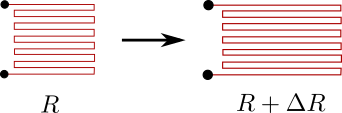
\includegraphics[scale=0.5]{stretched_gauge.png}

This is an exaggerated picture so the change is  very small...

\end{multicols}

{\tiny Images: T.Hill}
}


% Section I - Frame II:
\frame{
\frametitle{\sectiontitleI}

The {\PN Gauge Factor} is typically used instead of the physical parameters. \vspcc

\scalebox{1}{$GF \equiv \frac{\delta R/R}{\delta L/L}=\frac{\delta R/R}{\epsilon_a}$}\vspcc

This number relates the relative change in resistance to the measured strain. \vspc

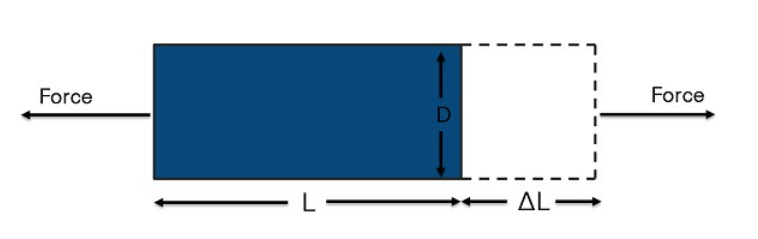
\includegraphics[scale=.25]{strain_fig2.png}

{\tiny Images: \href{https://www.ni.com/en-us/innovations/white-papers/07/measuring-strain-with-strain-gages.html}{NI}}
}

% Section II:
\section{\sectiontitleII}

% Section II - Frame I:
\frame{
\frametitle{\sectiontitleII}



\begin{multicols}{2}

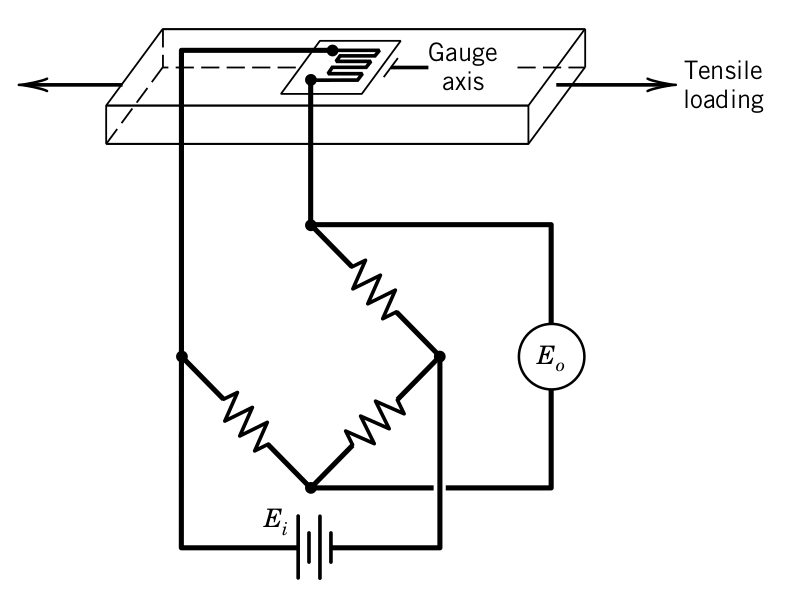
\includegraphics[scale=.25]{gauged_beam_bridge.png} \vspace{15mm} 

A {\PR transducer} converts the sensed information into a detectable signal. The signal might be mechanical, electrical, optical, or may take any other form that can be meaningfully recorded.

\end{multicols}

{\tiny Text. Images: Theory and Design for Mechanical Measurements}
}

% Section II - Frame II:
\frame{
\frametitle{\sectiontitleII}

\begin{multicols}{2}

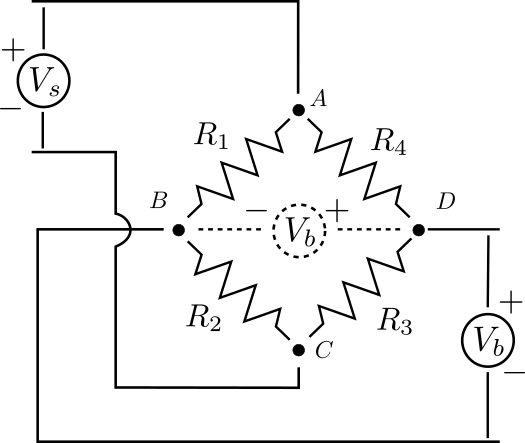
\includegraphics[scale=.35]{bridge_circuit.png} \vspace{15mm} 

How does the bridge circuit work as a transducer? \vspc Use KVL and the voltage divider rule find the relationship between the two voltages. \vspc



\scalebox{1}{$V_b=\left( \frac{R_3}{R_3+R_4}-\frac{R_2}{R_1+R_2}\right)\times V_s$}

\end{multicols}
 
{\tiny Images: T.Hill}
}


% Section III:
\section{\sectiontitleIII}

% Section I - Frame III:
\frame{
\frametitle{\sectiontitleIII}

If all four resistors are equal the bridge voltage will equal zero and the bridge is said it be {\B balanced}. 
One or more resistors in the circuit is replaced by a strain gauge and bridge voltage is used as a measure of change in resistance and therefore strain. \vspc
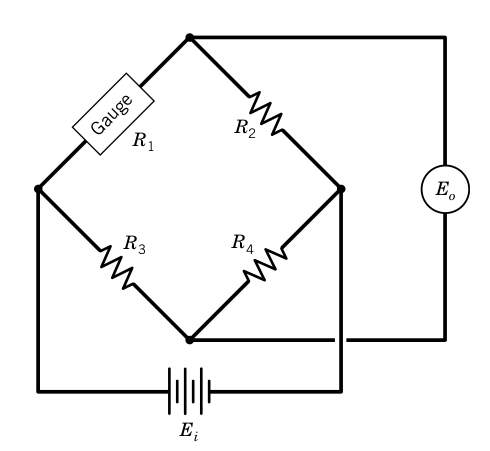
\includegraphics[scale=.2]{gauge_in_bridge_quarter.png} 

This gives a linear {\PR calibration curve} with a convenient {\R zero offset}. \vspc 
{\tiny Text. Images: Theory and Design for Mechanical Measurements}
}

% Section IV:
\section{\sectiontitleIV}

% Section IV - Frame I:
\frame{
\frametitle{\sectiontitleIV}

\begin{multicols}{2}

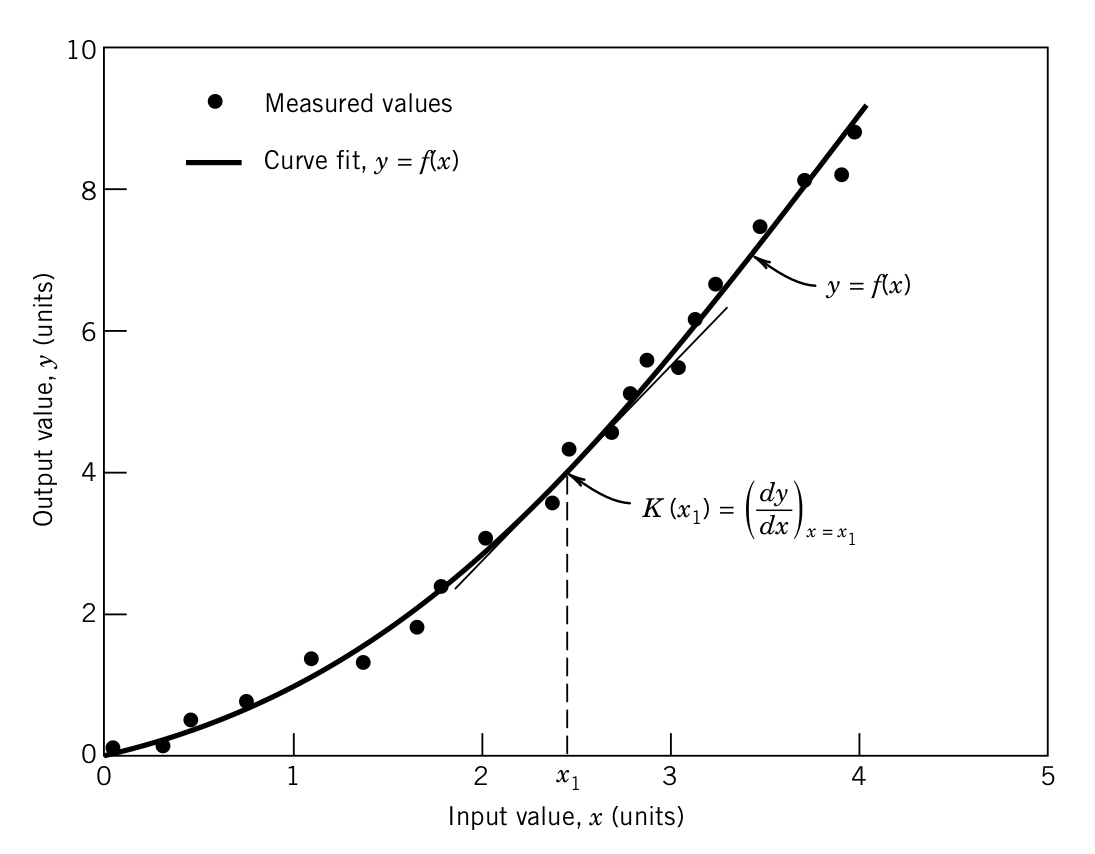
\includegraphics[scale=.14]{calibration_curve.png} 

\small
Assume $R=120\Omega$ for all resistors and the bridge is balanced in a condition of zero strain. What is the {\PN static sensitivity} of the gauge and bridge circuit described? \vspc

\scalebox{1}{K=}\vspc

\end{multicols}


{\tiny Text. Images: Theory and Design for Mechanical Measurements}
}

% Section IV - Frame II:
\frame{
\frametitle{\sectiontitleIV}

}
	
% Section IV - Frame III:
\frame{
\frametitle{\sectiontitleIV}

}
\end{document}





